\subsection{Results}
\label{subsec:molecular_dynamics_results}

The Langevin dynamics simulations were performed with the following parameters: unitary mass $m = 1$ and viscosity $\eta = 1$, and time integration step $d t = 0.01$. We only considered two values for the density, namely, $\rho = (0.25, 0.75)$, and to check for finite-size effects, we performed simulations with two different system sizes $N = (1600, 6400)$. \textcolor{red}{I have compared the results, and I don't see any dependence, however, I'm not sure how to show this}.

To study the dependence of the dynamics on the initial configuration, we performed simulations starting from three possible initial configurations. First, we generated the initial orientations uniformly at random; second,  we aligned all particles along the $z$ axis; and third, particles of even index were oriented along, and of odd index against $z$ axis. We refer to these configurations as ``random'', ``co-aligned'' and ``counter-aligned'', respectively. Commonly for three cases, the particle coordinates were obtained as for the Monte Carlo simulations.

We start by analyzing the relaxation of the order parameter $S$ defined in Eq.~\eqref{eq:nematic_order_parameter} to the equilibrium value. The results are shown in \figref{fig:op_relaxation}. The squares, circles and triangles correspond to ``random'', ``co-aligned'' and ``counter-aligned'' initial configurations, respectively.

First thing to note is that irrespectively of any other parameter, for ``counter-aligned'' and ``random'' initial configurations the relaxation follows the same path.
The notable distinction between relaxation of the order parameters at high $(\rho = 0.75)$ and low $(\rho = 0.25)$ density is that for the low density ``re-orientation'' occurs fast for any given $k_BT$, and due to that the relaxation from ``co-aligned'' initial configuration follows the same path as two other. Additionally, the results suggest power law behavior for any $k_BT$. This is not the case for high density, as we see in \figref{fig:op_relaxation}. For the high $k_BT \geq 1.5$ the behavior qualitatively similar to that for the case of low density. For the low $k_BT \le 1.5$ we can distinguish relaxation path for the ``co-aligned'' and two other initial configurations, and results suggests exponential relaxation of order parameter to equilibrium values.

Essentially, system have two timescales, one for ``re-orientation'' (equilibration of amount of particles pointing along and against $z$ axis), and the other for ``alignment'' (equilibration of distribution of projections of particles dipole moments, which corresponds to equilibration of order parameter). The former is shorter then the latter, but the difference decreases with decrease in $k_BT$ and increase in density.

\begin{figure*}[t]
\centering
\begin{minipage}[c]{0.32\textwidth}
	\centering
	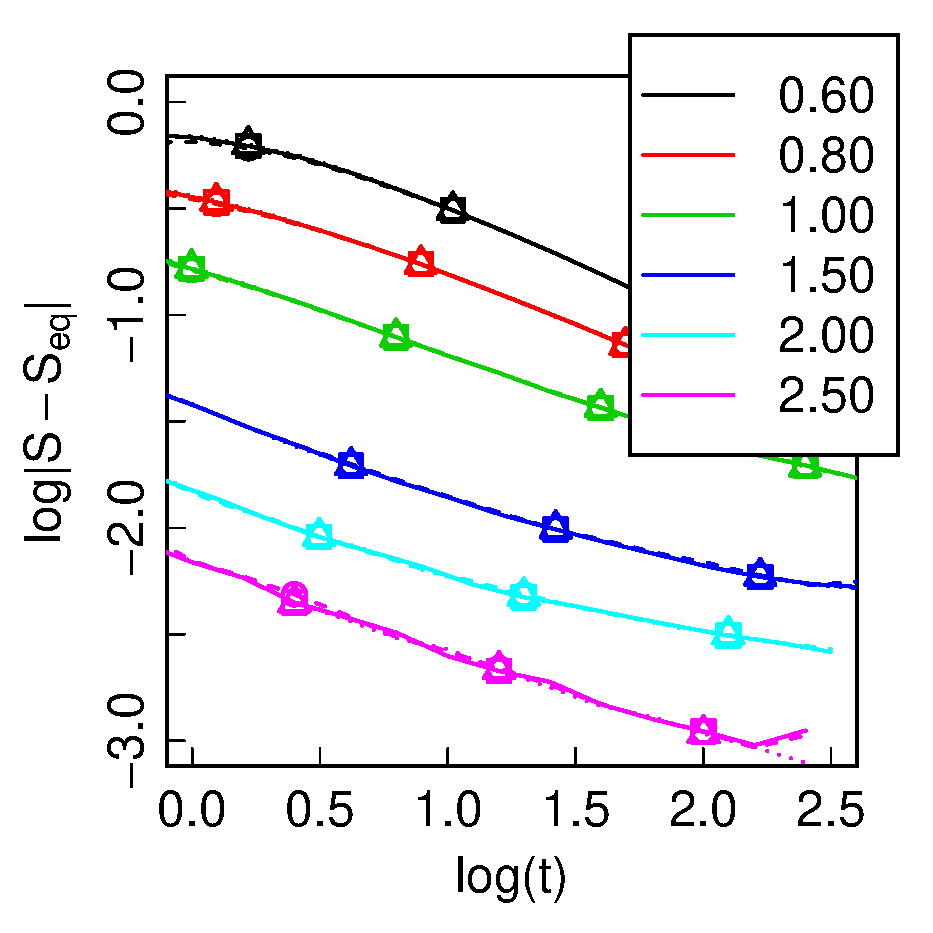
\includegraphics[width=\textwidth]{Images/relax_op_25}
\end{minipage}
\begin{minipage}[c]{0.32\textwidth}
	\centering
	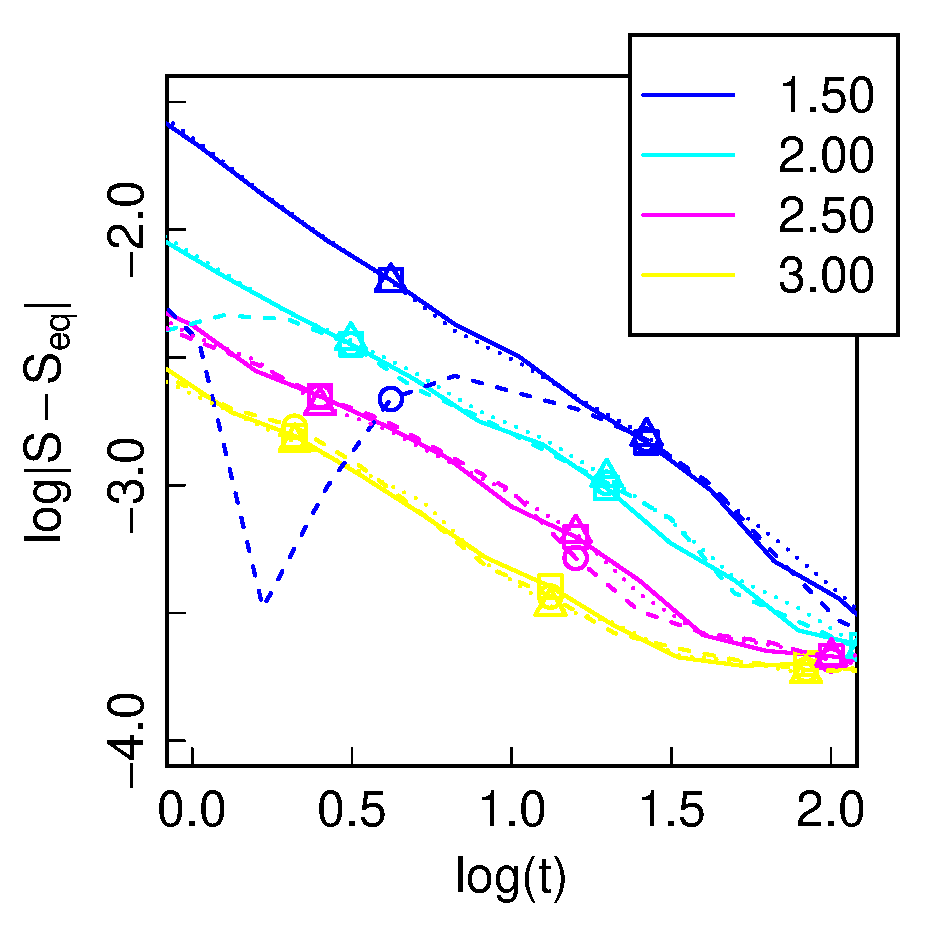
\includegraphics[width=\textwidth]{Images/relax_op_75}
\end{minipage}
\begin{minipage}[c]{0.32\textwidth}
	\centering
	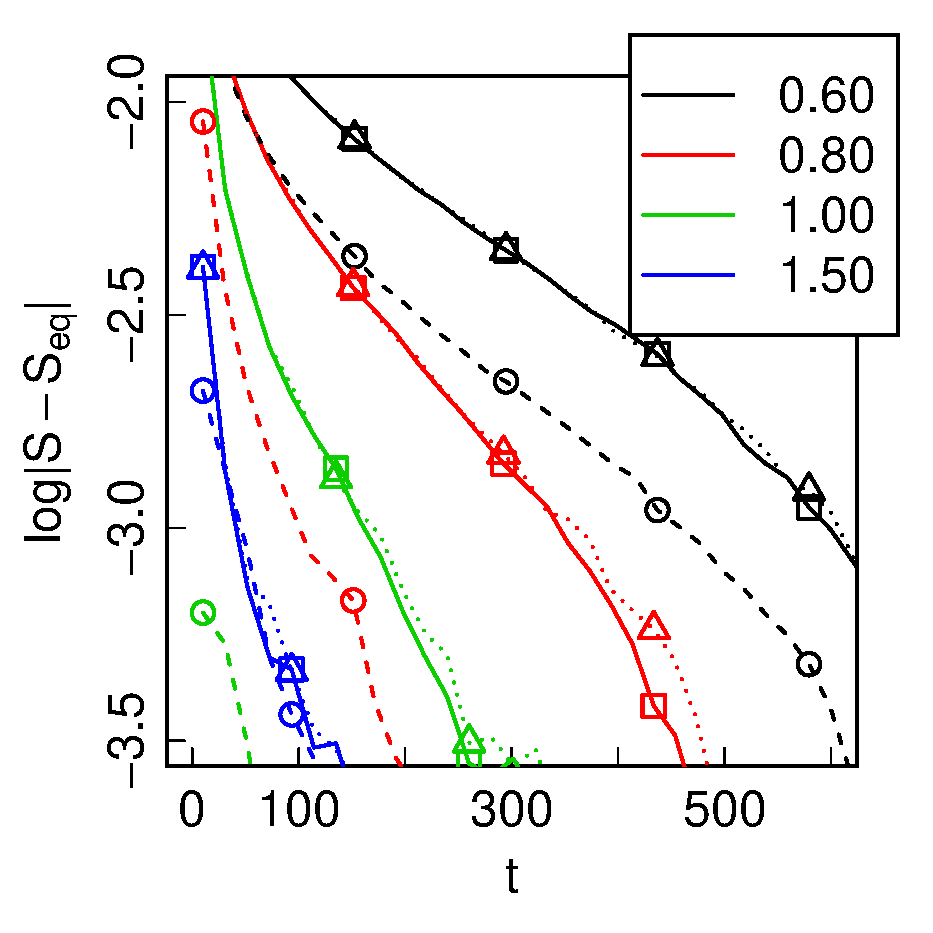
\includegraphics[width=\textwidth]{Images/relax_op_75_exp}
\end{minipage}
	\caption{Relaxation of order parameter to the equilibrium values for densities $\rho = 0.25$ (left) and $\rho = 0.75$, (middle and right) respectively. The squares, circles and triangles denote ``random'', ``co-aligned'' and ``counter-aligned'' initial configurations, respectively. Color indicates $k_BT$. The results are obtained on $500$ samples of $N = 6400$.}
	\label{fig:op_relaxation}
\end{figure*}

To check if simulations are loosing memory of initial configuration, we measure autocorrelation function of a particle orientation:
\begin{equation}
\label{eq:autocorrelation_ld}
	C(t) = \langle\cos\theta_i(t) \cdot \cos\theta_i(0)\rangle
\end{equation}
here $\theta_i(0)$ is the orientation of a particle $i$ at the beginning of simulation and $\theta_i(t)$ is the orientation of the same particle in the same sample at the time $t$. The ensemble-averaging is done over all particles and samples.

The results presented in the Fig.~\ref{fig:autocorrelation}. clearly shows the exponential tail for any given combination of parameters. However for short time scale the behavior isn't exponential, although in that case the relaxation is faster than the exponential regime, as we can clearly see in case of $k_BT = 0.8$ and $\rho = 0.25$ at the left of Fig.~\ref{fig:autocorrelation}. The relaxation time steadily increases with $k_BT$. Additionally we want to note that ``random'' initial configuration de-correlates faster than ``co-aligned'', albeit slower than ``counter-aligned'' configurations.

\begin{figure}[t]
\centering
	\begin{minipage}[c]{0.7\columnwidth}
		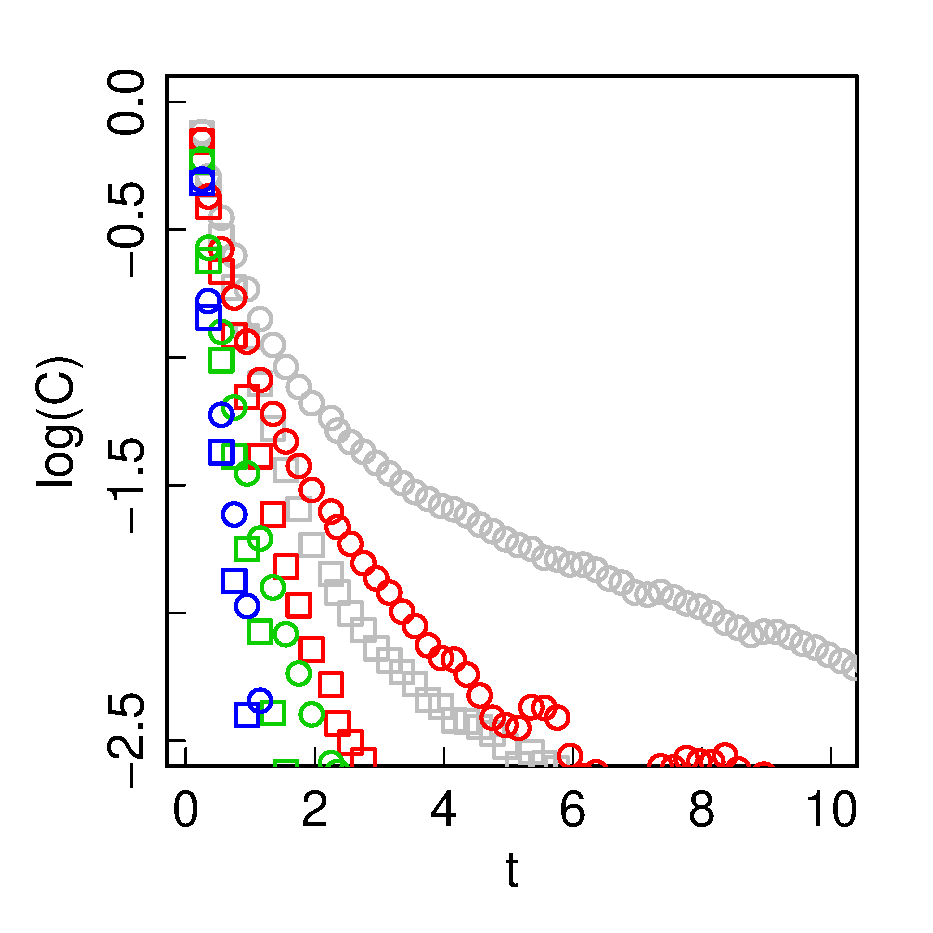
\includegraphics[width=\textwidth]{Images/Autocors_25}
	\end{minipage}
	\begin{minipage}[c]{0.7\columnwidth}
		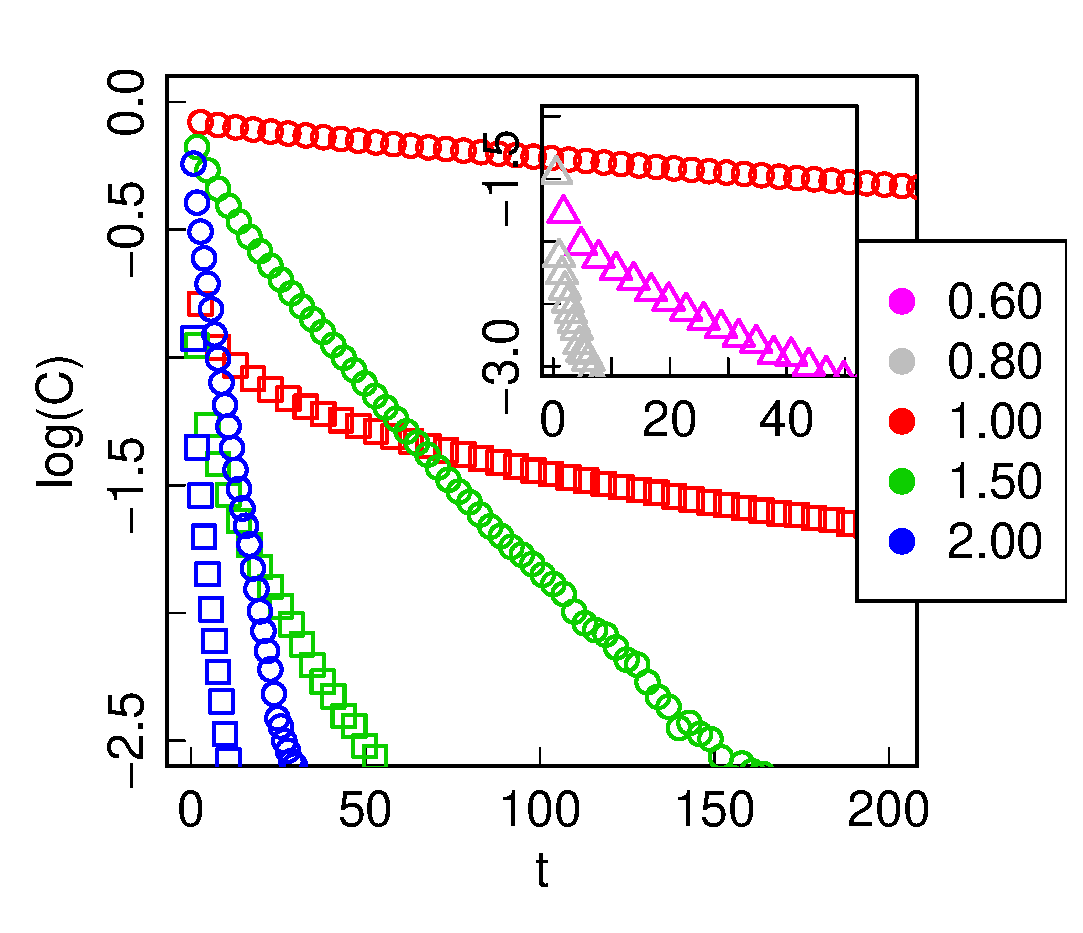
\includegraphics[width=\textwidth]{Images/Autocors_75}
	\end{minipage}
	\caption{Time dependence of particles autocorrelation for $\rho = 0.25$ (top) and $\rho = 0.75$ (bottom). The squares, circles and triangles denote ``random'', ``co-aligned'' and ``counter-aligned'' initial configurations, respectively. The color codes $k_BT$ values. The results are obtained on $500$ samples of $N = 6400$.}
	\label{fig:autocorrelation}
\end{figure}

To gain more insight on the system dynamics, we look into particle-particle correlations in the orientation.
Two neighboring particles are considered to be part of the same aggregate if
\begin{equation}
\label{eq:chains_definition}
\begin{cases}
	|z_i - z_j| \leq l \\
	\theta_{i, j} \leq \alpha \text{ \textbf{or} } \theta_{i, j} \geq \pi - \alpha
\end{cases}
\end{equation}
where $l$ is a predefined separation distance after which particles are ``unchained'', and second condition considers only particles that are oriented along the same direction, within a certain angle $\alpha$. We define one to be ``right'' chain if all the particles satisfy $\theta_i \leq \alpha$, ``left'' if $\theta_i \geq \pi - \alpha$, and ``undefined'' in all other cases. Then we can measure the probability of two neighbouring chains to be ``left-left'' (``LL'') or ``left-right'' (``LR''), etc. The ``undefined'' chains can consist only of solitary particles, and so we suggest to treat all particles as separate chains (i.e. $l \ll D$)

The main results are shown in Fig.~\ref{fig:prob_relaxation}.

First of all, we need to note that due to the symmetry of the system potential, the equilibrium results for the pairs ``LL'' -- ``RR'' and ``LR'' -- ``RL'' are the same, accounting for the statistical error.

Similar to order parameter, for the low density the relaxation for any of the given orientation pairs suggests power law behavior. Also is important that there is little difference in slope for co-aligned and counter-aligned orientation pairs, as well as little influence of the $k_BT$. The respective pairs (``LL'' -- ``RR'' and ``LR'' -- ``RL'') quickly relax to the same values and then the relaxation follows the same path.

For the high density the behavior is more complicated. First of all, the results suggest the exponential relaxation for prevalent (in this case ``RR'') orientation pair, with the power strongly dependent on the $k_BT$. On the other hand, the opposite to prevalent orientation pair (``LL'') relaxes differently after the initial moments and before the relaxation to the same values. We can see that most clearly for the $k_BT = 2.5$ in the $t \in (5, 15)$ range.

Another observation is that co-aligned orientation pairs relaxes slower then counter-aligned. It can be attributed to less favorable energy configuration of the latter, and therefore much lesser representation on the equilibrium.

\begin{figure*}[t]
\centering
\begin{minipage}[c]{0.8\columnwidth}
	\includegraphics[width=\textwidth]{Images/Particle_probs_25}
\end{minipage}
\begin{minipage}[c]{0.8\columnwidth}
	\includegraphics[width=\textwidth]{Images/Particle_probs_75}
\end{minipage}

\begin{minipage}[c]{0.8\columnwidth}
	\includegraphics[width=\textwidth]{Images/Particle_probs_relaxation_25}
\end{minipage}
\begin{minipage}[c]{0.8\columnwidth}
	\includegraphics[width=\textwidth]{Images/Particle_probs_relaxation_75}
\end{minipage}
	\caption{Particle-particle correlations in the orientation (top) and their relaxation to the equilibrium values (bottom), for $\rho = 0.25$ (left) and $\rho = 0.75$ (right). Lines show the equilibrium results, however, the pairs ``LL'' -- ``RR'' and ``LR'' -- ``RL'' values are indistinguishable at this scale. The simulations start from co-aligned initial configuration. The results are obtained on $500$ samples of $N = 6400$.}
	\label{fig:prob_relaxation}
\end{figure*}


